
\begin{exercice}[2019 -- 2020]
On utilise la structure de donnée suivante :

\begin{lstlisting}
Structure Cellule:
    Entier valeur
    Cellule suivante

Structure File:
    Cellule premiere
\end{lstlisting}

Donner un algorithme qui prend en entrée une liste chaînée et un entier $k$ et supprime les $k$ premiers éléments de la liste.

Par exemple, si la liste est 
\scalebox{.8}{
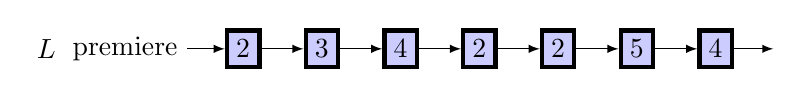
\begin{tikzpicture}[>=latex]
\node(L) at (-2,0){$L$};
\node(Prem) at (-1,0){premiere};

\node(T1)[draw, ultra thick, fill=blue!20, rectangle] at (0.5,0) {2};
\node(T2)[draw, ultra thick, fill=blue!20, rectangle] at (1.5,0) {3};
\node(T3)[draw, ultra thick, fill=blue!20, rectangle] at (2.5,0) {4};
\node(T4)[draw, ultra thick, fill=blue!20, rectangle] at (3.5,0) {2};
\node(T5)[draw, ultra thick, fill=blue!20, rectangle] at (4.5,0) {2};
\node(T6)[draw, ultra thick, fill=blue!20, rectangle] at (5.5,0) {5};
\node(T7)[draw, ultra thick, fill=blue!20, rectangle] at (6.5,0) {4};

\draw (Prem.east) edge[->] (T1.west);
\draw (T1.east) edge[->] (T2.west);
\draw (T2.east) edge[->] (T3.west);
\draw (T3.east) edge[->] (T4.west);
\draw (T4.east) edge[->] (T5.west);
\draw (T5.east) edge[->] (T6.west);
\draw (T6.east) edge[->] (T7.west);
\draw (T7.east) edge[->] ++(.5,0);
\end{tikzpicture}
}

Le résultat après le passage de l'algorithme avec $k=3$ sera 
\scalebox{.8}{
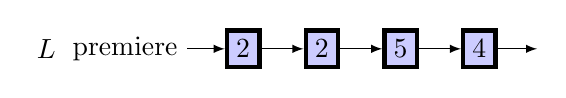
\begin{tikzpicture}[>=latex]
\node(L) at (1,0){$L$};
\node(Prem) at (2,0){premiere};

\node(T4)[draw, ultra thick, fill=blue!20, rectangle] at (3.5,0) {2};
\node(T5)[draw, ultra thick, fill=blue!20, rectangle] at (4.5,0) {2};
\node(T6)[draw, ultra thick, fill=blue!20, rectangle] at (5.5,0) {5};
\node(T7)[draw, ultra thick, fill=blue!20, rectangle] at (6.5,0) {4};

\draw (Prem.east) edge[->] (T4.west);

\draw (T4.east) edge[->] (T5.west);
\draw (T5.east) edge[->] (T6.west);
\draw (T6.east) edge[->] (T7.west);
\draw (T7.east) edge[->] ++(.5,0);
\end{tikzpicture}
}

\textbf{Solution}


\begin{lstlisting}
Algo
Input : Liste L, entier k
Procédé :
c <- L.premiere
i <- 0
Tant que i < k et c != None:
    i <- i+1
    c <- c.suivante
L.premiere <- c
\end{lstlisting}


Question donnée au partiel 1 2019-2020, résultats obtenus :

\begin{tabular}{|c|c|c|c|c|}
\hline
A & B & C & D & E \\ \hline
55\% & 30\% & 7\% & 4\% & 4\% \\ \hline
\end{tabular} 



\end{exercice}